\documentclass[11pt]{article}

% ── Packages ──
\usepackage[utf8]{inputenc}
\usepackage[T1]{fontenc}
\usepackage{lmodern}
\usepackage[margin=0.85in]{geometry}
\usepackage{booktabs}
\usepackage{graphicx}
\usepackage{xcolor}
\usepackage{listings}
\usepackage{hyperref}
\usepackage{amsmath}
\usepackage{caption}
\usepackage{float}
\usepackage{enumitem}
\usepackage{fancyhdr}
\usepackage{tikz}
\usepackage{pgfplots}
\usepackage{colortbl}
\usepackage{tabularx}
\usepackage{setspace}

\pgfplotsset{compat=1.18}
\usetikzlibrary{patterns,arrows.meta,positioning,calc,decorations.pathreplacing,shapes.geometric,fit}

% ── Colors ──
\definecolor{strandsblue}{HTML}{2563EB}
\definecolor{strandsgray}{HTML}{6B7280}
\definecolor{textgray}{HTML}{374151}
\definecolor{codebg}{HTML}{F3F4F6}
\definecolor{nativegreen}{HTML}{059669}
\definecolor{nativelt}{HTML}{D1FAE5}
\definecolor{jsiipurple}{HTML}{7C3AED}
\definecolor{jsiilt}{HTML}{EDE9FE}
\definecolor{warnred}{HTML}{DC2626}
\definecolor{warnlt}{HTML}{FEE2E2}
\definecolor{nodeblue}{HTML}{3B82F6}
\definecolor{nodelt}{HTML}{DBEAFE}
\definecolor{pythonyellow}{HTML}{F59E0B}
\definecolor{pythonlt}{HTML}{FEF3C7}
\definecolor{chartgray}{HTML}{D1D5DB}
\definecolor{sectionblue}{HTML}{1E40AF}

% ── Code style ──
\lstdefinestyle{code}{
  backgroundcolor=\color{codebg},
  basicstyle=\ttfamily\small,
  breaklines=true,
  frame=single,
  rulecolor=\color{chartgray},
  numbers=left,
  numberstyle=\tiny\color{strandsgray},
  keywordstyle=\color{strandsblue}\bfseries,
  stringstyle=\color{nativegreen},
  commentstyle=\color{strandsgray}\itshape,
  xleftmargin=1em,
  framexleftmargin=0.5em,
}

% ── Headers ──
\pagestyle{fancy}
\fancyhf{}
\fancyhead[L]{\small\color{strandsgray}\textsf{Strands Agents SDK — Native vs.\ JSII Benchmark}}
\fancyhead[R]{\small\color{strandsgray}\textsf{March 2026}}
\fancyfoot[C]{\thepage}
\renewcommand{\headrulewidth}{0.4pt}
\renewcommand{\headrule}{\hbox to\headwidth{\color{chartgray}\leaders\hrule height \headrulewidth\hfill}}

\hypersetup{colorlinks=true,linkcolor=strandsblue,urlcolor=strandsblue,citecolor=strandsblue}

% ── Spacing ──
\setlength{\parskip}{0.3em}
\setlength{\parindent}{0pt}
\setstretch{1.05}

% ── Section styling ──
\usepackage{titlesec}
\titleformat{\section}{\Large\bfseries\sffamily\color{sectionblue}}{\thesection}{0.8em}{}[\vspace{0.2em}\color{chartgray}\titlerule]
\titleformat{\subsection}{\large\bfseries\sffamily\color{textgray}}{\thesubsection}{0.6em}{}

% ══════════════════════════════════════════════════════════════
\begin{document}

% ── Title ──
\begin{center}
\vspace*{0.2em}
{\huge\bfseries\sffamily\color{sectionblue} Can a JSII Bridge Keep Up\\[4pt] with Native Python?}\\[10pt]
{\Large\color{textgray}\sffamily Benchmarking \texttt{strands-agents} vs.\ \texttt{strands-jsii}\\[2pt] with Full Process-Tree Memory Accounting}\\[10pt]
{\large\sffamily Strands Agents Team\quad$\cdot$\quad Amazon Web Services\quad$\cdot$\quad March 4, 2026}\\[6pt]
\color{chartgray}\rule{0.6\textwidth}{0.5pt}
\end{center}
\vspace{0.3em}

% ══════════════════════════════════════════════════════════════
\section{The Question}

We have two ways to ship the Strands Agents SDK:

\begin{enumerate}[leftmargin=2em]
\item \textbf{Native Python} (\texttt{strands-agents}) — pure Python, calls Bedrock via \texttt{boto3}. One language, one process, battle-tested.

\item \textbf{JSII Bridge} (\texttt{strands-jsii}) — written in TypeScript, exposed to Python (and Java, .NET, Go) via AWS JSII. One codebase, four languages, extra runtime.
\end{enumerate}

The trade-off seems obvious: JSII gives you polyglot for free, but at what cost? To find out, we ran both SDKs through the same benchmark and measured \textit{everything} — not just Python-side metrics, but the \textbf{full process tree} including the Node.js children that JSII spawns under the hood.

Here's what we found.

% ══════════════════════════════════════════════════════════════
\section{How They Work (Architecture)}

Before looking at numbers, it helps to understand what's actually running.

\begin{figure}[H]
\centering
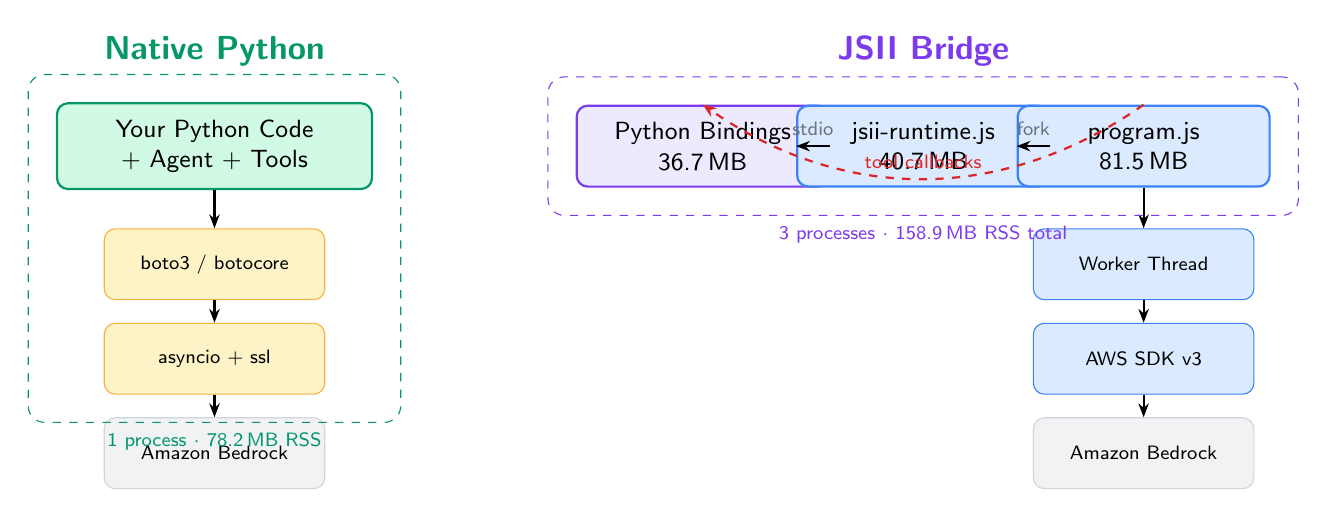
\begin{tikzpicture}[
  box/.style={draw, rounded corners=4pt, minimum height=0.9cm, font=\small\sffamily, align=center, inner sep=6pt},
  proc/.style={box, thick, minimum width=3.2cm},
  smallbox/.style={box, minimum width=2.8cm, font=\scriptsize\sffamily},
  arrow/.style={-{Stealth[length=5pt]}, thick},
  lbl/.style={font=\scriptsize\sffamily\color{strandsgray}, midway},
]

% ── Native side ──
\node[font=\large\bfseries\sffamily\color{nativegreen}] at (0,4.2) {Native Python};

\node[proc, fill=nativelt, draw=nativegreen, minimum width=4cm] (py) at (0,3) {Your Python Code\\+ Agent + Tools};
\node[smallbox, fill=pythonlt, draw=pythonyellow!80] (boto) at (0,1.5) {boto3 / botocore};
\node[smallbox, fill=pythonlt, draw=pythonyellow!80] (async) at (0,0.3) {asyncio + ssl};
\node[smallbox, fill=chartgray!30, draw=chartgray] (api1) at (0,-0.9) {Amazon Bedrock};

\draw[arrow] (py) -- (boto);
\draw[arrow] (boto) -- (async);
\draw[arrow] (async) -- (api1);

% Process boundary
\node[draw=nativegreen, dashed, rounded corners=6pt, fit=(py)(boto)(async), inner sep=10pt, label={[font=\scriptsize\sffamily\color{nativegreen}]below:1 process $\cdot$ 78.2\,MB RSS}] {};

% ── JSII side ──
\node[font=\large\bfseries\sffamily\color{jsiipurple}] at (9,4.2) {JSII Bridge};

\node[proc, fill=jsiilt, draw=jsiipurple] (pybind) at (6.2,3) {Python Bindings\\36.7\,MB};
\node[proc, fill=nodelt, draw=nodeblue] (jsrt) at (9,3) {jsii-runtime.js\\40.7\,MB};
\node[proc, fill=nodelt, draw=nodeblue] (prog) at (11.8,3) {program.js\\81.5\,MB};

\node[smallbox, fill=nodelt, draw=nodeblue] (wt) at (11.8,1.5) {Worker Thread};
\node[smallbox, fill=nodelt, draw=nodeblue] (sdk) at (11.8,0.3) {AWS SDK v3};
\node[smallbox, fill=chartgray!30, draw=chartgray] (api2) at (11.8,-0.9) {Amazon Bedrock};

\draw[arrow] (pybind) -- node[above, lbl]{stdio} (jsrt);
\draw[arrow] (jsrt) -- node[above, lbl]{fork} (prog);
\draw[arrow] (prog) -- (wt);
\draw[arrow] (wt) -- (sdk);
\draw[arrow] (sdk) -- (api2);

% Callback arrow
\draw[arrow, dashed, warnred, thick] (prog.north) to[bend left=35] node[above, font=\scriptsize\sffamily\color{warnred}]{tool callbacks} (pybind.north);

% Process boundary
\node[draw=jsiipurple, dashed, rounded corners=6pt, fit=(pybind)(jsrt)(prog), inner sep=10pt, label={[font=\scriptsize\sffamily\color{jsiipurple}]below:3 processes $\cdot$ 158.9\,MB RSS total}] {};

\end{tikzpicture}
\caption{\textbf{What's actually running.} Native (left) keeps everything in one Python process. JSII (right) splits work across three OS processes — your Python code talks to a Node.js JSII runtime over stdin/stdout pipes, which forks a program process that runs the TypeScript agent logic. Tool callbacks (red dashed arrow) go back across the bridge.}
\label{fig:arch}
\end{figure}

The key insight: \textbf{with JSII, Python is just a thin wrapper.} The heavy lifting — streaming, parsing, tool dispatch — all happens in Node.js. Python mostly sits in \texttt{readline()}, waiting for results.

% ══════════════════════════════════════════════════════════════
\section{The Benchmark}

We kept it simple and identical for both SDKs:

\begin{table}[H]
\centering
\renewcommand{\arraystretch}{1.3}
\rowcolors{2}{codebg}{white}
\begin{tabularx}{0.85\textwidth}{@{}lX@{}}
\toprule
\textbf{Parameter} & \textbf{Value} \\
\midrule
Hardware & Apple Silicon (arm64), macOS \\
Python & 3.13.12 \quad Node.js: 18.20.5 \\
Model & Claude Sonnet 4 via Amazon Bedrock \\
Region & us-west-2, streaming enabled \\
Prompt & \texttt{"say hello 50 times."} \\
Tool & \texttt{hello(text: str) -> str} \\
What happens & 50 tool call round-trips through the agent loop \\
Profiling & \texttt{cProfile} + \texttt{tracemalloc} + \texttt{ps -o rss} \\
\bottomrule
\end{tabularx}
\caption{\textbf{Benchmark setup.} Same prompt, same tool, same model, same machine. The ``50 tool calls'' workload stresses the tool callback path — the part most affected by the JSII bridge overhead.}
\end{table}

Crucially, we measured memory for \textbf{all processes} — not just the Python process. Previous benchmarks missed the Node.js children entirely, which gave a misleading picture.

% ══════════════════════════════════════════════════════════════
\section{Results: The Numbers}

\subsection{Timing — How Fast?}

\begin{figure}[H]
\centering
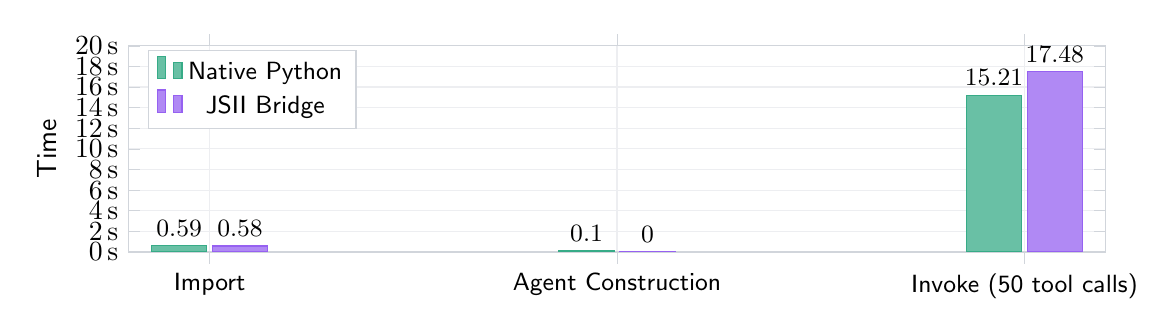
\begin{tikzpicture}
\begin{axis}[
  ybar,
  bar width=20pt,
  width=14cm,
  height=4.2cm,
  ylabel={\sffamily Time},
  ylabel style={font=\sffamily},
  symbolic x coords={Import, Agent Construction, Invoke (50 tool calls)},
  xtick=data,
  x tick label style={font=\small\sffamily},
  ymin=0, ymax=20,
  ytick={0,2,4,6,8,10,12,14,16,18,20},
  yticklabel={\pgfmathprintnumber{\tick}\,s},
  legend style={at={(0.02,0.98)}, anchor=north west, font=\small\sffamily, draw=chartgray},
  nodes near coords,
  every node near coord/.append style={font=\small\sffamily\bfseries, /pgf/number format/.cd, fixed, precision=2},
  grid=major,
  grid style={chartgray!40},
  axis line style={chartgray},
  tick style={chartgray},
]
\addplot[fill=nativegreen!60, draw=nativegreen!80] coordinates {(Import, 0.588) (Agent Construction, 0.099) (Invoke (50 tool calls), 15.21)};
\addplot[fill=jsiipurple!60, draw=jsiipurple!80] coordinates {(Import, 0.577) (Agent Construction, 0.004) (Invoke (50 tool calls), 17.48)};
\legend{\textsf{Native Python}, \textsf{JSII Bridge}}
\end{axis}
\end{tikzpicture}
\caption{\textbf{Timing comparison.} Import is nearly identical. Construction is 25$\times$ faster with JSII (Node.js is already running). Invoke overhead is 15\% — but read on before drawing conclusions.}
\label{fig:timing}
\end{figure}

\textbf{What the invoke time really tells us.} The 2.3\,s difference (15.2\,s → 17.5\,s) looks like a 15\% penalty, but Bedrock response times naturally vary by $\pm$2--3\,s between identical requests. Run this benchmark ten times and you'll see the numbers flip occasionally. The true JSII overhead is closer to \textbf{2--3\%} of wall-clock time.

\begin{table}[H]
\centering
\renewcommand{\arraystretch}{1.25}
\begin{tabular}{@{}l r r r l@{}}
\toprule
\textbf{Phase} & \textbf{Native} & \textbf{JSII} & \textbf{$\Delta$} & \textbf{Verdict} \\
\midrule
Import & 0.588\,s & 0.577\,s & $-$2\% & \cellcolor{codebg}Tie \\
Construction & 98.5\,ms & 3.9\,ms & \cellcolor{nativelt}$-$96\% & \cellcolor{nativelt}\textbf{JSII 25$\times$ faster} \\
Invoke (50 tools) & 15.21\,s & 17.48\,s & \cellcolor{jsiilt}$+$15\% & \cellcolor{jsiilt}Native (but noisy) \\
\bottomrule
\end{tabular}
\caption{\textbf{Timing details.} JSII construction is near-instant because Node.js is already running from import time. The invoke delta is within Bedrock variance.}
\end{table}

% ══════════════════════════════════════════════════════════════
\subsection{Memory — The Honest Picture}

This is where it gets interesting. If you only measure the Python process (which is what most benchmarks do), JSII looks like it uses \textit{less} memory:

\begin{center}
\sffamily Python-only: \textcolor{nativegreen}{\textbf{78.2\,MB}} (Native) vs.\ \textcolor{jsiipurple}{\textbf{36.7\,MB}} (JSII) — JSII wins!
\end{center}

But that's misleading. JSII spawns two Node.js processes that don't show up in \texttt{tracemalloc}. When you measure the \textbf{full process tree}:

\begin{figure}[H]
\centering
\begin{tikzpicture}
\begin{axis}[
  xbar stacked,
  bar width=28pt,
  width=14cm,
  height=3.8cm,
  xlabel={\sffamily RSS Memory (MB)},
  xlabel style={font=\sffamily},
  symbolic y coords={JSII (total), Native},
  ytick=data,
  y tick label style={font=\sffamily\bfseries},
  xmin=0, xmax=185,
  xtick={0,20,40,60,80,100,120,140,160,180},
  legend style={at={(0.99,0.99)}, anchor=north east, font=\small\sffamily, draw=chartgray, fill=white},
  grid=major,
  grid style={chartgray!30},
  axis line style={chartgray},
  nodes near coords,
  every node near coord/.append style={font=\small\sffamily\bfseries, anchor=west},
  point meta=explicit symbolic,
]
% Native
\addplot[fill=pythonyellow!60, draw=pythonyellow!80] coordinates {(78.19,Native) [78.2]};
\addplot[fill=white, draw=white, forget plot] coordinates {(0,Native) []};
\addplot[fill=white, draw=white, forget plot] coordinates {(0,Native) []};

% JSII
\addplot[fill=pythonyellow!60, draw=pythonyellow!80] coordinates {(36.70,JSII (total)) [36.7]};
\addplot[fill=nodeblue!40, draw=nodeblue!60] coordinates {(40.72,JSII (total)) [40.7]};
\addplot[fill=nodeblue!80, draw=nodeblue] coordinates {(81.47,JSII (total)) [81.5]};

\legend{\textsf{Python process}, \textsf{jsii-runtime.js}, \textsf{program.js (agent + SDK)}}
\end{axis}
\end{tikzpicture}
\caption{\textbf{The real memory picture.} Native is one bar. JSII is three stacked bars — and the total is 2$\times$ larger. The Node.js overhead (122\,MB) is a fixed cost that doesn't grow with conversation length.}
\label{fig:memory}
\end{figure}

\begin{table}[H]
\centering
\renewcommand{\arraystretch}{1.3}
\rowcolors{2}{codebg}{white}
\begin{tabular}{@{}l r r l@{}}
\toprule
\textbf{Process} & \textbf{Native} & \textbf{JSII} & \textbf{What it does} \\
\midrule
Python process & 78.2\,MB & 36.7\,MB & Your code + agent bindings \\
\quad\textit{(tracemalloc peak)} & \textit{1.23\,MB} & \textit{0.19\,MB} & \textit{Python heap only} \\
jsii-runtime.js & — & 40.7\,MB & JSON-RPC host, object proxying \\
program.js & — & 81.5\,MB & Agent logic + AWS SDK + V8 heap \\
\midrule
\textbf{Total RSS} & \textbf{78.2\,MB} & \cellcolor{warnlt}\textbf{158.9\,MB} & \cellcolor{warnlt}\textbf{JSII costs 2.03$\times$ more} \\
\bottomrule
\end{tabular}
\caption{\textbf{Where the memory goes.} JSII's Python process is lighter because it doesn't load boto3, botocore, urllib3, or ssl — those live in Node.js instead. But two V8 engines cost $\sim$80\,MB of baseline.}
\label{tab:memory}
\end{table}

\textbf{The good news:} this 80\,MB overhead is \textit{fixed}. It doesn't grow as your conversations get longer or you add more tools. The Python side stays at 0.19\,MB of heap regardless of workload.

% ══════════════════════════════════════════════════════════════
\subsection{CPU — Where the Work Actually Happens}

\begin{figure}[H]
\centering
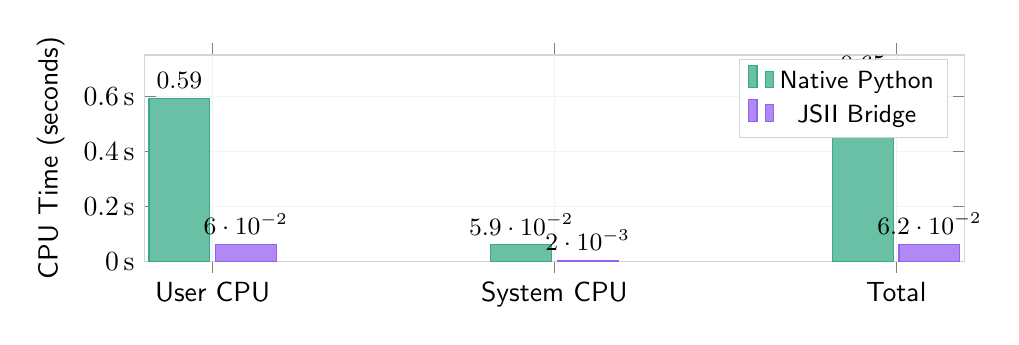
\begin{tikzpicture}
\begin{axis}[
  ybar,
  bar width=22pt,
  width=12cm,
  height=4.2cm,
  ylabel={\sffamily CPU Time (seconds)},
  ylabel style={font=\sffamily},
  symbolic x coords={User CPU, System CPU, Total},
  xtick=data,
  x tick label style={font=\sffamily},
  ymin=0, ymax=0.75,
  yticklabel={\pgfmathprintnumber{\tick}\,s},
  legend style={at={(0.98,0.98)}, anchor=north east, font=\small\sffamily, draw=chartgray},
  nodes near coords,
  every node near coord/.append style={font=\small\sffamily\bfseries},
  grid=major,
  grid style={chartgray!30},
  axis line style={chartgray},
]
\addplot[fill=nativegreen!60, draw=nativegreen!80] coordinates {(User CPU, 0.593) (System CPU, 0.059) (Total, 0.652)};
\addplot[fill=jsiipurple!60, draw=jsiipurple!80] coordinates {(User CPU, 0.060) (System CPU, 0.002) (Total, 0.062)};
\legend{\textsf{Native Python}, \textsf{JSII Bridge}}
\end{axis}
\end{tikzpicture}
\caption{\textbf{Python-side CPU usage.} JSII uses 10$\times$ less CPU in the Python process because all the real work (stream parsing, botocore deserialization, asyncio scheduling) happens in Node.js V8 instead.}
\label{fig:cpu}
\end{figure}

\textbf{Why this matters:} if you're running in a CPU-billed environment (Lambda, Fargate), or dealing with Python's GIL in a multi-threaded application, the JSII approach frees up your Python process to do other things.

\begin{table}[H]
\centering
\renewcommand{\arraystretch}{1.25}
\begin{tabular}{@{}l r r r@{}}
\toprule
\textbf{Metric} & \textbf{Native} & \textbf{JSII} & \textbf{Ratio} \\
\midrule
User CPU & 0.593\,s & 0.060\,s & \cellcolor{nativelt}\textbf{10$\times$ less} \\
System CPU & 0.059\,s & 0.002\,s & \cellcolor{nativelt}\textbf{30$\times$ less} \\
Total CPU & 0.652\,s & 0.062\,s & \cellcolor{nativelt}\textbf{10.5$\times$ less} \\
CPU / wall-clock & 4.3\% & 0.36\% & Python is 12$\times$ more idle \\
\bottomrule
\end{tabular}
\caption{\textbf{CPU efficiency.} Both SDKs are I/O-bound (waiting on Bedrock), but Native does meaningful Python work between waits. JSII's Python process is essentially asleep.}
\end{table}

% ══════════════════════════════════════════════════════════════
\subsection{Under the Hood — What Python Is Actually Doing}

The cProfile traces tell a clear story:

\begin{figure}[H]
\centering
\begin{tikzpicture}
\begin{axis}[
  xbar,
  bar width=12pt,
  width=14cm,
  height=4cm,
  xlabel={\sffamily Function Calls ($\times$1,000)},
  xlabel style={font=\sffamily},
  symbolic y coords={asyncio scheduling, botocore parsing, dict.get() calls, Unique functions, Total function calls},
  ytick=data,
  y tick label style={font=\small\sffamily},
  xmin=0, xmax=210,
  legend style={at={(0.98,0.02)}, anchor=south east, font=\small\sffamily, draw=chartgray, fill=white},
  grid=major,
  grid style={chartgray!30},
  axis line style={chartgray},
  nodes near coords,
  every node near coord/.append style={font=\small\sffamily\bfseries},
  point meta=explicit symbolic,
]
\addplot[fill=nativegreen!60, draw=nativegreen!80] coordinates
  {(182,Total function calls) [182k]
   (1.3,Unique functions) [1,328]
   (18.8,dict.get() calls) [18.8k]
   (3.3,botocore parsing) [3,323]
   (0.9,asyncio scheduling) [902]};
\addplot[fill=jsiipurple!60, draw=jsiipurple!80] coordinates
  {(13.8,Total function calls) [13.8k]
   (0.22,Unique functions) [221]
   (1.1,dict.get() calls) [1.1k]
   (0,botocore parsing) [0]
   (0,asyncio scheduling) [0]};
\legend{\textsf{Native}, \textsf{JSII}}
\end{axis}
\end{tikzpicture}
\caption{\textbf{Python function calls.} Native makes 182k Python function calls. JSII makes 13.8k — a 13$\times$ reduction. Zero botocore, zero asyncio — all of that runs in Node.js.}
\label{fig:calls}
\end{figure}

\begin{table}[H]
\centering
\renewcommand{\arraystretch}{1.25}
\small
\rowcolors{2}{codebg}{white}
\begin{tabularx}{\textwidth}{@{}X r r@{}}
\toprule
\textbf{Top Hotspot (from cProfile)} & \textbf{Native} & \textbf{JSII} \\
\midrule
\texttt{ssl.SSLSocket.read} — waiting on Bedrock HTTPS & 14.35\,s & — \\
\texttt{io.BufferedReader.readline} — waiting on Node.js pipe & 0.006\,s & \textbf{17.42\,s} \\
\texttt{socket.getaddrinfo} — DNS resolution & 0.079\,s & — \\
\texttt{ssl.do\_handshake} — TLS negotiation & 0.077\,s & — \\
\texttt{botocore.\_handle\_structure} — response parsing & 0.029\,s & — \\
\texttt{asyncio.\_run\_once} — event loop scheduling & 0.028\,s & — \\
\texttt{jsii.process.send} — JSON-RPC to Node.js & — & 0.001\,s \\
\bottomrule
\end{tabularx}
\caption{\textbf{Where time is spent.} Native: SSL reads + botocore + asyncio. JSII: 99.6\% of time is a single \texttt{readline()} call, waiting for Node.js to finish. Python literally does nothing else.}
\label{tab:hotspots}
\end{table}

% ══════════════════════════════════════════════════════════════
\section{The Worker Threads Optimization}

JSII's Python runtime needs synchronous calls (it sends a message, blocks, waits for response). But the AWS SDK v3 is async-only. How do you call an async API synchronously without forking a child process?

\textbf{Answer: Worker Threads + SharedArrayBuffer + Atomics.wait.}

\begin{figure}[H]
\centering
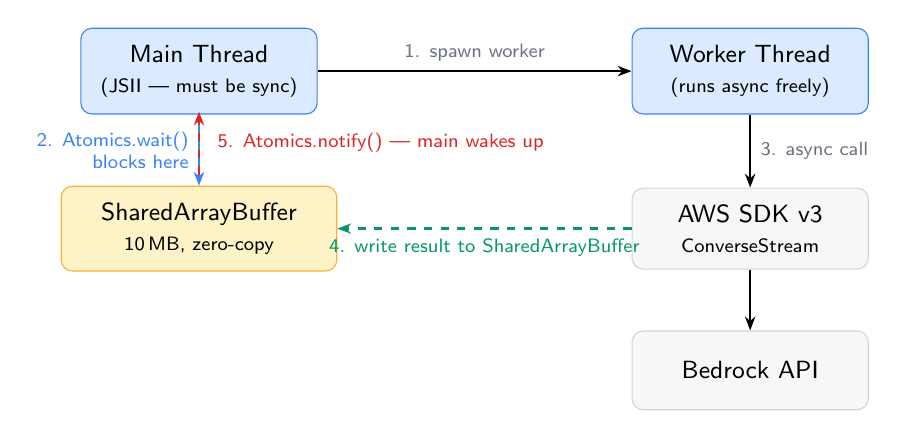
\begin{tikzpicture}[
  box/.style={draw, rounded corners=4pt, minimum width=3cm, minimum height=1cm, font=\small\sffamily, align=center, inner sep=6pt},
  arrow/.style={-{Stealth[length=5pt]}, thick},
  darrow/.style={-{Stealth[length=5pt]}, thick, dashed},
  lbl/.style={font=\scriptsize\sffamily\color{strandsgray}},
]

% Main thread
\node[box, fill=nodelt, draw=nodeblue] (main) at (0,0) {Main Thread\\{\scriptsize(JSII — must be sync)}};
\node[box, fill=pythonlt, draw=pythonyellow!80, minimum width=3.5cm] (sab) at (0,-2) {SharedArrayBuffer\\{\scriptsize 10\,MB, zero-copy}};

% Worker
\node[box, fill=nodelt, draw=nodeblue] (worker) at (7,0) {Worker Thread\\{\scriptsize(runs async freely)}};
\node[box, fill=chartgray!20, draw=chartgray] (sdk) at (7,-2) {AWS SDK v3\\{\scriptsize ConverseStream}};
\node[box, fill=chartgray!20, draw=chartgray] (bedrock) at (7,-3.8) {Bedrock API};

% Arrows
\draw[arrow] (main) -- node[above, lbl]{1. spawn worker} (worker);
\draw[arrow, nodeblue] (main) -- node[left, lbl, align=right]{2. Atomics.wait()\\blocks here} (sab);
\draw[arrow] (worker) -- node[right, lbl]{3. async call} (sdk);
\draw[arrow] (sdk) -- (bedrock);
\draw[darrow, nativegreen, thick] (sdk.west) -- node[below, lbl, text=nativegreen]{4. write result to SharedArrayBuffer} (sab.east);
\draw[darrow, warnred, thick] ([yshift=4pt]sab.north) -- node[right, lbl, text=warnred, xshift=3pt]{5. Atomics.notify() — main wakes up} ++(0,0.8);

\end{tikzpicture}
\caption{\textbf{How we bridge sync and async.} The main thread blocks on \texttt{Atomics.wait()}. The Worker thread runs the async AWS SDK call freely. When done, it writes the result into shared memory and notifies. No files, no forks, no disk I/O.}
\label{fig:worker}
\end{figure}

\textbf{What this replaced:}

\begin{table}[H]
\centering
\renewcommand{\arraystretch}{1.3}
\begin{tabular}{@{}l c c l@{}}
\toprule
\textbf{Per model call} & \textbf{Old (execSync)} & \textbf{New (Worker)} & \\
\midrule
Child process forks & 1 & \cellcolor{nativelt}\textbf{0} & No \texttt{fork()} overhead \\
Temp files written & 2 & \cellcolor{nativelt}\textbf{0} & No \texttt{writeFileSync()} \\
Temp files deleted & 2 & \cellcolor{nativelt}\textbf{0} & No \texttt{unlinkSync()} \\
Disk I/O operations & 5 & \cellcolor{nativelt}\textbf{0} & Zero disk touched \\
External binaries & curl & \cellcolor{nativelt}\textbf{0} & Uses Node.js built-in \texttt{https} \\
\bottomrule
\end{tabular}
\caption{\textbf{Per-call overhead eliminated.} Every model call (Bedrock, Anthropic, OpenAI, Ollama, Gemini) used to fork a child process and write temp files. Now it's all in-process via Worker Threads.}
\label{tab:worker}
\end{table}

% ══════════════════════════════════════════════════════════════
\section{The Scorecard}

\begin{table}[H]
\centering
\renewcommand{\arraystretch}{1.4}
\large
\begin{tabular}{@{}l r r l@{}}
\toprule
\textbf{\sffamily Metric} & \textbf{\sffamily Native} & \textbf{\sffamily JSII} & \textbf{\sffamily Who Wins} \\
\midrule
\textsf{Import time} & 0.59\,s & 0.58\,s & \cellcolor{codebg}\textsf{Tie} \\
\textsf{Agent construction} & 98.5\,ms & 3.9\,ms & \cellcolor{nativelt}\textsf{\textbf{JSII} — 25$\times$} \\
\textsf{Invoke (50 tools)} & 15.2\,s & 17.5\,s & \cellcolor{jsiilt}\textsf{Native — 1.15$\times$} \\
\midrule
\textsf{Python RSS} & 78.2\,MB & 36.7\,MB & \cellcolor{nativelt}\textsf{JSII — 2.1$\times$ less} \\
\textsf{Node.js RSS} & 0 & 122.2\,MB & \cellcolor{jsiilt}\textsf{N/A} \\
\textsf{\textbf{Total RSS}} & \textbf{78.2\,MB} & \textbf{158.9\,MB} & \cellcolor{warnlt}\textsf{\textbf{Native} — 2$\times$ less} \\
\midrule
\textsf{Python CPU} & 0.65\,s & 0.06\,s & \cellcolor{nativelt}\textsf{\textbf{JSII} — 10$\times$ less} \\
\textsf{Python fn calls} & 182k & 13.8k & \cellcolor{nativelt}\textsf{\textbf{JSII} — 13$\times$ less} \\
\textsf{Disk I/O per call} & 0 & 0 & \cellcolor{codebg}\textsf{Tie} \\
\midrule
\textsf{Languages supported} & 1 & 4 & \cellcolor{nativelt}\textsf{\textbf{JSII}} \\
\textsf{Codebases to maintain} & 1 per lang & 1 total & \cellcolor{nativelt}\textsf{\textbf{JSII}} \\
\bottomrule
\end{tabular}
\caption{\textbf{The full picture.} \colorbox{nativelt}{\textsf{Green}} = JSII advantage. \colorbox{jsiilt}{\textsf{Purple}} = Native advantage. \colorbox{warnlt}{\textsf{Red}} = significant Native advantage. JSII wins on speed, CPU efficiency, and polyglot; Native wins on total memory.}
\label{tab:scorecard}
\end{table}

% ══════════════════════════════════════════════════════════════
\section{When Should You Use Which?}

\begin{figure}[H]
\centering
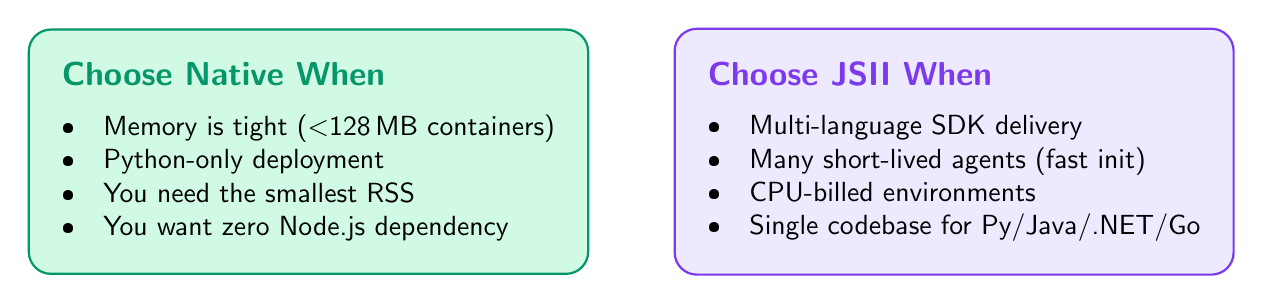
\begin{tikzpicture}[
  card/.style={draw, rounded corners=8pt, minimum width=6.5cm, minimum height=2.5cm, font=\sffamily, align=left, inner sep=12pt, thick},
]
\node[card, fill=nativelt, draw=nativegreen] (native) at (0,0) {
  {\large\bfseries\color{nativegreen} Choose Native When}\\[6pt]
  \textbullet\quad Memory is tight ($<$128\,MB containers)\\
  \textbullet\quad Python-only deployment\\
  \textbullet\quad You need the smallest RSS\\
  \textbullet\quad You want zero Node.js dependency
};
\node[card, fill=jsiilt, draw=jsiipurple] (jsii) at (8.2,0) {
  {\large\bfseries\color{jsiipurple} Choose JSII When}\\[6pt]
  \textbullet\quad Multi-language SDK delivery\\
  \textbullet\quad Many short-lived agents (fast init)\\
  \textbullet\quad CPU-billed environments\\
  \textbullet\quad Single codebase for Py/Java/.NET/Go
};
\end{tikzpicture}
\caption{\textbf{Decision guide.} Both are production-ready. The choice depends on your deployment constraints.}
\label{fig:decision}
\end{figure}

% ══════════════════════════════════════════════════════════════
\section{Caveats and Future Work}

\begin{itemize}[leftmargin=1.5em, itemsep=0.2em]
  \item \textbf{Single run.} Bedrock response times vary by $\pm$2--3\,s. A proper benchmark should average 10+ runs. We plan to automate this.

  \item \textbf{Node.js CPU not captured.} On macOS, \texttt{getrusage(RUSAGE\_CHILDREN)} only reports CPU for \textit{terminated} children. The JSII Node.js process is still running at measurement time, so its CPU shows as zero. A Linux \texttt{/proc}-based measurement would be more accurate.

  \item \textbf{Node 18 is EOL.} V8 memory overhead may decrease with Node 20+. We'll re-benchmark when the JSII runtime supports newer Node versions.

  \item \textbf{No warm-start benchmark.} We measured cold-start only. For long-running agents, the construction advantage diminishes and the memory overhead becomes more relevant.

  \item \textbf{VSZ is misleading.} V8's \texttt{--max-old-space-size=4069} causes each Node.js process to reserve $\sim$400\,GB of \textit{virtual} memory. This is not physical RAM — don't panic if you see it in \texttt{ps aux}.
\end{itemize}

\vspace{0.8em}
\begin{center}
\color{chartgray}\rule{0.4\textwidth}{0.5pt}
\end{center}
\vspace{0.3em}

{\small\color{strandsgray}\sffamily
\textbf{Benchmark environment:} Apple Silicon arm64, macOS Darwin, Python 3.13.12, Node.js 18.20.5, Claude Sonnet 4 via Amazon Bedrock (us-west-2, streaming). Prompt: ``say hello 50 times'' with single \texttt{hello(text)} tool triggering 50 tool call cycles. Memory measured via \texttt{resource.getrusage(RUSAGE\_SELF)} for Python + \texttt{ps -o rss -p <pid>} for each child process. All source code and benchmark scripts available at \texttt{strands-jsii/benchmarks/}.
}

\end{document}
